\documentclass[a4paper]{article}

\usepackage[T1]{fontenc}
\usepackage[utf8x]{inputenc}

\usepackage[a4paper]{geometry}
\geometry{verbose,tmargin=3cm,bmargin=3cm,lmargin=2cm,rmargin=2cm,headheight=2cm,headsep=1cm,footskip=2cm}

\usepackage{fancyhdr}
\usepackage{enumerate}
\usepackage{adjustbox}
\pagestyle{fancy}
\setlength{\parskip}{\medskipamount}
\setlength{\parindent}{0pt}
\usepackage{graphicx}

\makeatletter

\usepackage{subcaption}
\usepackage{varwidth}
\usepackage{float} 
\usepackage{color}
\usepackage{lastpage}
\usepackage{indentfirst}

\usepackage{pgf}
\usepackage{tikz}
\usetikzlibrary{arrows,automata, shapes, positioning, calc}

\lhead[lh-even]{Edgar Vedvik (edgarmv)\\ Informatikk (BIT)}
\chead[ch-even]{TDT4205 Kompilatorteknikk\\ Problem Set 6 }
\rhead[rh-even]{\today}

\lfoot[lf-even]{}
\cfoot[cf-even]{Side \thepage{} av \pageref{LastPage}}
\rfoot[rf-even]{}

\tikzset{
    -|/.style={to path={-| (\tikztotarget)}},
    |-/.style={to path={|- (\tikztotarget)}},
}

\date{}

\makeatother

\usepackage[english]{babel}

\begin{document}


\thispagestyle{fancy}

\section{Theory}
\subsection{Control flow graphs}
    In figure 1 I assume that the code is:\\
    \\
    for ( a ; b ; c) \{\}\\
    d;\\
    e;\\
    \\
    not:\\
    \\
    for ( a ; b ; c)\\
    \phantom{x}\hspace{1 em} d;\\
    e;\\
\begin{figure}[ht]
    \begin{minipage}[b]{0.5\linewidth}
        \centering
        \begin{tikzpicture}
            [->, >=stealth', auto, node distance=1cm, semithick,
            itemset/.style={rectangle, align=center, draw=black}]

            \node[itemset,minimum size=1cm] (e) {e};
            \node[itemset,minimum size=1cm] (d) [above = of e] {d};
            \node[itemset,minimum size=1cm] (b) [above = of d] {b};
            \node[itemset,minimum size=1cm] (c) [left = of b] {c};
            \node[itemset,draw,minimum size=1cm] (a) [above = of b] {a};

            \draw (a) edge (b);
            \draw (b) edge [bend left=10] (c);
            \draw (c) edge [bend left=10] (b);
            \draw (b) edge (d);
            \draw (d) edge (e);
        \end{tikzpicture}
        \caption{for ( a ; b ; c ) d ; e ;}
        \vspace{4ex}
    \end{minipage}%%
    \begin{minipage}[b]{0.5\linewidth}
        \centering
        \begin{tikzpicture}
            [->, >=stealth', auto, node distance=1cm, semithick,
            itemset/.style={rectangle, align=center, draw=black}]

            \node[itemset,minimum size=1cm] (a) {a};
            \node[itemset,minimum size=1cm] (b) [below = of a] {b};
            \node[itemset,minimum size=1cm] (d) [below = of b] {d};
            \node[itemset,minimum size=1cm] (c) [left = of d] {c};
            \node[itemset,minimum size=1cm] (e) [below = of d] {e};

            \draw (a) edge (b);
            \draw (b) edge (d);
            \draw (d) edge (c);
            \draw (c) |- (b);
            \draw (b) -- +(2,0) |- (e);
        \end{tikzpicture}
        \caption{a ; while ( b ) \{ d ; c ; \} e ;}
        \vspace{4ex}
    \end{minipage}
    \begin{minipage}[b]{0.5\linewidth}
        \centering
        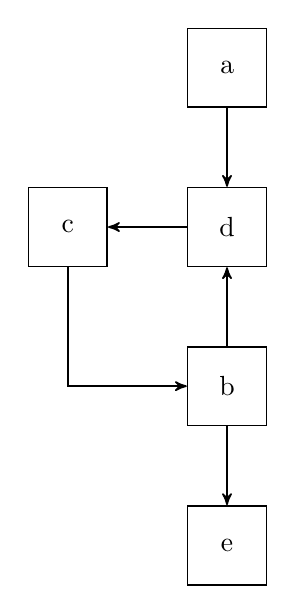
\begin{tikzpicture}
            [->, >=stealth', auto, node distance=1cm, semithick,
            itemset/.style={rectangle, align=center, draw=black}]

            \node[itemset,minimum size=1cm] (a) {a};
            \node[itemset,minimum size=1cm] (d) [below = of a] {d};
            \node[itemset,minimum size=1cm] (c) [left = of d] {c};
            \node[itemset,minimum size=1cm] (b) [below = of d] {b};
            \node[itemset,minimum size=1cm] (e) [below = of b] {e};

            \draw (a) edge (d);
            \draw (d) edge (c);
            \draw (c) |- (b);
            \draw (b) edge (d);
            \draw (b) edge (e);
        \end{tikzpicture}
        \caption{a ; do \{ d ; c ; \} while ( b ); e ;}
    \end{minipage}
\end{figure}
\subsection{Optimizations}

\subsubsection{Copy propagation}
        \begin{figure}[H]
            \centering
            \begin{varwidth}{0.45\textwidth}
                \begin{enumerate}[1.]
                    \item a=1
                    \item b=2
                    \item c=3
                    \item d=a+x
                    \item e=b+c
                    \item f=e
                    \item {\color{red}$\mathbf{g=f}$}
                    \item g=d+y
                    \item a=b+c
                \end{enumerate}
                \caption{Before}
            \end{varwidth}
            \begin{varwidth}{0.45\textwidth}
                \begin{enumerate}[1.]
                    \item a=1
                    \item b=2
                    \item c=3
                    \item d=a+x
                    \item e=b+c
                    \item f=e
                    \item {\color{red}$\mathbf{g=e}$}
                    \item g=d+y
                    \item a=b+c
                \end{enumerate}
                \caption{After}
            \end{varwidth}
        \end{figure}
\subsubsection{Common subexpression elimination}
        \begin{figure}[H]
            \centering
            \begin{varwidth}[b]{0.45\linewidth}
                \begin{enumerate}[1.]
                    \item a=1
                    \item b=2
                    \item c=3
                    \item d=a+x
                    \item {\color{red}$\mathbf{e=b+c}$}
                    \item f=e
                    \item g=f
                    \item g=d+y
                    \item {\color{red}$\mathbf{a=b+c}$}
                \end{enumerate}
                \caption{Before}
            \end{varwidth}
            \begin{varwidth}[b]{0.45\linewidth}
                \begin{enumerate}[1.]
                    \item a=1
                    \item b=2
                    \item c=3
                    \item d=a+x
                    \item {\color{red}$\mathbf{t1=b+c}$}
                    \item {\color{red}$\mathbf{e=t1}$}
                    \item f=e
                    \item g=f
                    \item g=d+y
                    \item {\color{red}$\mathbf{a=t1}$}
                \end{enumerate}
                \caption{After}
            \end{varwidth}
        \end{figure}
\subsubsection{Constant propagation}
        \begin{flushleft}
        Assuming only constant propagation, not constant folding.
        \end{flushleft}
        \centering
        \begin{figure}[H]
            \centering
            \begin{varwidth}[b]{0.45\textwidth}
                \begin{enumerate}[1.]
                    \item $a=1$
                    \item $b=2$
                    \item $c=3$
                    \item {\color{red}$\mathbf{d=a+x}$}
                    \item {\color{red}$\mathbf{e=b+c}$}
                    \item $f=e$
                    \item $g=f$
                    \item $g=d+y$
                    \item {\color{red}$\mathbf{a=b+c}$}
                \end{enumerate}
                \caption{Before}
            \end{varwidth}
            \begin{varwidth}[b]{0.45\textwidth}
                \begin{enumerate}[1.]
                    \item a=1
                    \item b=2
                    \item c=3
                    \item {\color{red}$\mathbf{d=1+x}$}
                    \item {\color{red}$\mathbf{e=2+3}$}
                    \item f=e
                    \item g=f
                    \item g=d+y
                    \item {\color{red}$\mathbf{a=2+3}$}
                \end{enumerate}
                \caption{After}
            \end{varwidth}
        \end{figure}
\end{document}
